\documentclass{article}

\usepackage[francais]{babel}
\def\printlandscape{\special{landscape}}    % Works with dvips.
%\usepackage{pstricks,pst-node,pst-tree}
%\usepackage{amssymb}
\usepackage[utf8]{inputenc}
\usepackage[T1]{fontenc} 
\usepackage{fancybox} % for shadow and Bitemize
\usepackage{alltt}
\usepackage{graphicx}
\usepackage{caption} 
\usepackage{textgreek}

%\usepackage{epsfig}
\usepackage{fullpage}
%\usepackage{fancyhdr}
%\usepackage{moreverb}
%\usepackage{xspace}
\usepackage[colorlinks,hyperindex,bookmarks,linkcolor=blue,citecolor=blue,urlcolor=blue]{hyperref}
\usepackage{array,multirow,makecell}
\setcellgapes{1pt}
\makegapedcells
\newcolumntype{R}[1]{>{\raggedleft\arraybackslash }b{#1}}
\newcolumntype{L}[1]{>{\raggedright\arraybackslash }b{#1}}
\newcolumntype{C}[1]{>{\centering\arraybackslash }b{#1}}
\usepackage{wrapfig}
\usepackage{epsf}
\usepackage{framed}

\usepackage{fancyvrb}
\usepackage{xcolor}
\definecolor{Zgris}{rgb}{0.87,0.85,0.85}


\newcommand{\HRule}{\rule{\linewidth}{0.5mm}}

\newsavebox{\BBbox}

\newenvironment{DDbox}[1]{
	\begin{lrbox}{\BBbox}\begin{minipage}{\linewidth}}
		{\end{minipage}\end{lrbox}\noindent\colorbox{Zgris}{\usebox{\BBbox}} \\
		[.5cm]}

\title{Rapport du TER GMIN401 :\\ \textbf{Intégration et optimisation d’algorithmes de classifications supervisées pour Weka}}

\author{Par : ALIJATE Mehdi - NEGROS Hadrien - TURKI Batoul}

\date{31 Janvier 2014}

         
\begin{document}

\begin{titlepage}

  \begin{center}

    % Partie superieure
    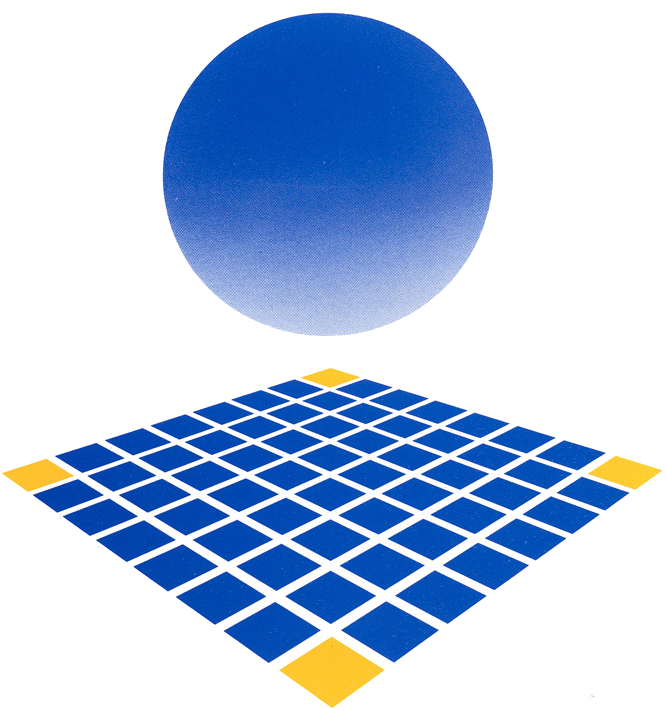
\includegraphics[width=0.30\textwidth]{logo_um2}~\\[1cm]    

    \textsc{\LARGE Université Montpellier II \\ -- Facultés des sciences --}\\[1.5cm]
       
    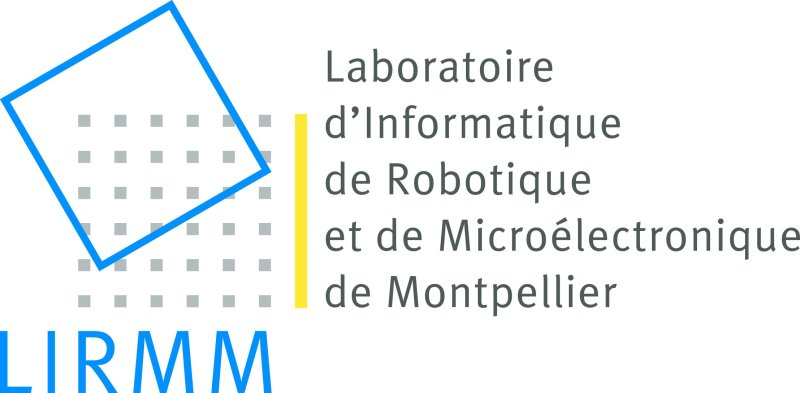
\includegraphics[width=0.40\textwidth]{lirmm}~\\[1cm]    
    \textsc{\huge Travail d'étude et de recherche}\\[0.5cm]

    % Titre
    \HRule \\[0.4cm]
    { \huge \bfseries Intégration et optimisation d’algorithmes de classifications supervisées pour Weka}\\[0.4cm]
    \HRule \\[1.5cm]

    % Auteurs et encandrants
    \begin{minipage}{0.4\textwidth}
      \begin{flushleft} \large
        \emph{Auteurs :}\\
        Mehdi \textsc{Alijate} \\
        Hadrien \textsc{Negros} \\
        Batoul \textsc{Turki} \\   
      \end{flushleft}
    \end{minipage}
    \begin{minipage}{0.4\textwidth}
      \begin{flushright} \large
        \emph{Encadrant :} \\
        Flavien \textsc{Bouillot} \\
      \end{flushright}
    \end{minipage}
    \vfill

    % Partie inferieure
    {\large 21 Février 2014}

  \end{center}

\end{titlepage}
\tableofcontents

\begin{abstract}
	
Ce sujet vise à intégrer et à optimiser des algorithmes de classifications supervisées de documents dans la suite logiciel WEKA. Ces algorithmes sont issus de travaux de recherche menés récemment au sein du LIRMM.
\begin{center}
\href{https://github.com/sorgenh/TERWeka/}{https://github.com/sorgenh/TERWeka/}
\end{center}
\end{abstract}

\newpage 
%-----------------------------------------------------------
\section{Introduction}\label{sec:intro}
La classification de documents est le mécanisme consistant à classer automatiquement des ressources dans la classe prédéfinie lui correspondant le mieux.\\
Plusieurs formes de classifications existent (par genre, par opinion, par thème...etc), et se font via des algorithmes de classifications spécifiques. Ceux-ci se basent sur des méthodes principalement numériques (probabilistes), avec des algorithmes utilisant les mathématiques ou basés sur la recherche d'information. \\
Ce TER vise justement à intégrer des algorithmes de classifications supervisées de documents dans la suite logiciel WEKA\footnote{\href{http://www.cs.waikato.ac.nz/~ml/weka/}{Weka est une suite populaire de logiciels d'apprentissage automatique. Écrite en Java, développée à l'université de Waikato, Nouvelle-Zélande. Weka est un Logiciel libre disponible sous la Licence publique générale GNU.}}, se basant sur un nouveau modèle de classification à partir d'un faible nombre de documents, intégrant de nouvelles pondérations adaptées.\\
Tout d'abord, il faudra explorer l'API de WEKA, pour prendre en main le code source, la maniabilité des classes et explorer une méthode d'ajout d'un algorithme de classification. Ensuite, nous nous pencherons sur le développement des différentes classes en établissant une méthodologie concrétisant le travail mené au laboratoire du LIRMM, s'ensuivra une phase d'intégration et de tests.


%-----------------------------------------------------------

\section{Exploration de WEKA}
Après la réunion du 24/01/14, nous avons établi un plan de travail pour bien mener et répartir les tâches de ce TER. Il a été décidé de le diviser en trois grandes parties. La première, qui est décrite ci-dessous consiste à explorer et prendre en main l'API de WEKA, afin de pouvoir y rajouter les algorithmes que l'on aura développés lors de la deuxième partie, et qui seront testés et intégrés lors de la troisième.
\subsection{L'API Weka/Sources avec Eclipse}
Pour explorer l'API, nous nous sommes aidés de l'IDE Eclipse, qui permet facilement parcourir les sources d'une librairie externe. Après avoir étudié l'arborescence des classes de l'API, nous avons pu cibler les différentes classes et méthodes qui nous intéressent, et étudié leur fonctionnement. Nous nous sommes aidés de ce wiki \footnote{\href{http://weka.wikispaces.com/}{http://weka.wikispaces.com/}}.

\subsection{L'utilisation des classes}
Une fois familiarisés avec l'API Weka, nous avons creusé un peu plus du côté des classes qui pourraient nous être utiles pour ce TER. Il s'agit des certaines classes présentes dans le package{\scriptsize { \normalsize "weka.classifiers"}}. En effet, notre but étant d'intégrer des algorithmes de classification, il est utile de savoir comment ils tournent, ainsi que leur paramétrage et l'architecture pour organiser les ressources pour ces derniers.\\
Quelques tests ont été menés notamment pour bayes naif multinomial, que nous avons fait tourner sur différentes données, et avec différentes options.
\subsection{Ajout d'un algorithme dans Weka}\label{sec:algoW}
Après avoir étudié en détail la classe \textit{NaiveBayesMultinomial}, nous avons remarqué que le calcul des pondérations (dans l'implémentation de Weka, seule la mesure intra-classe Tf est utilisée) se fait dans la méthode \textbf{buildClassifier}. Nous allons donc créer une sous-classe de \textit{NaiveBayesMultinomial}, contenant une méthode surchargeant \textbf{buildClassifier} dans laquelle nous calculerons toutes les pondérations supplémentaires.\\
Une fois tout cela creusé et vu en détail, il faudra intégrer l'algorithme dans l'écosystème de Weka, c'est à dire pour le rendre disponible dans l'Explorateur, expérimentateur, etc . 
Weka prend en charge les classes dérivées dans le package, ceci est géré par le \textit{GenericPropertiesCreator}. Il faudra donc dire à Weka où trouver notre nouveau classificateur et il s'occupera de l'afficher dans la \textit{GenericObjectEditor}.\\
Nous y reviendrons plus en détails lors de la troisième étape de notre TER : L'intégration des algorithmes dans WEKA.
%-----------------------------------------------------------
\section{De nouvelles méthodes de classification}
Dans cette partie, nous allons vous présenter les différentes pondérations que nous allons utiliser pour construire nos classifieurs.
Nous allons d'abord définir les mesures intra-classe inspirées du TF-IDF, puis les mesures inter-classe développées au \textit{LIRMM}.
Ces mesures vont nous permettre de définir si un terme (un élément d'un document) est plus ou moins représentatif de la classe.\\Toutes ces mesures ont étés définies dans l'article \textit{De nouvelles pondérations adaptées à la classification de petits volumes de données textuelles. }\cite{RNTIB}.
\subsection{Pondérations intra-classe}
Les pondérations que nous définissons ci-dessous sont dites \textbf{intra-classe} car les différentes valeurs que nous utilisons pour les
calculer sont dépendantes d'une classe.
\subsubsection*{intra-classe document}
Cette mesure dépend du nombre de documents contenant le terme dans la classe.
  \[ inner\mbox{-}weight_{ij}^{Df} = \frac{DF_{ti}^j}{|d_{j}|}\]
  
      Avec:
  \begin{itemize}
  	\item $DF_{ti}^j$: Nombre de documents contenant le terme $t_i$ dans la classe $C_j$	
  	\item $|d_{j}|$: Nombre de documents dans $C_j$	
    \end{itemize}
\subsubsection*{intra-classe terme}
Cette mesure dépend du nombre d'occurrences du terme dans la classe.
\[   inner\mbox{-}weight_{ij}^{Tf} = \frac{TF_{ti}^j}{|n_{j}|}\]
  Avec:
\begin{itemize}
	\item $TF_{ti}^j$: Nombre d'occurrences du terme $t_i$ dans la classe $C_j$	
	\item $|n_{j}|$: Nombre de termes total dans la classe $C_j$	
  \end{itemize}
\subsection{Pondérations inter-classe}
Les pondérations inter-classes en revanche utilisent des valeurs calculées à partir de l'ensemble du corpus (depuis les classes extérieures à celle qui nous intéresse).
\subsubsection*{inter-classe terme}
Cette mesure dépend du nombre de classes contenant le terme.
\[inter\mbox{-}weight_{ij}^{class} = log_2 \frac{|C|}{C_{ti}}\]
Avec:
\begin{itemize}
	\item $|C|$: Nombre de classes			
	\item $C_{ti}$: Nombre de classes contenant le terme $t_i$
  \end{itemize}
\subsubsection*{inter-classe document}
Cette mesure dépend du nombre de documents extérieurs à la classe contenant le terme.
\[ inter\mbox{-}weight_{ij}^{doc} = log_2 \frac{|d \notin{C_j}|+1}{|d:t_i \notin{C_j}|+1}= log_2 \frac{|d|-|d \in{C_j}|+1}{|d:t_i|-|d:t_i \in{C_j}|+1}\]
 Avec:
\begin{itemize}
	\item $|d \notin  {C_j}|$: Nombre de documents n'appartenant pas à la classe $C_j$
	\item $|d:t_i \notin {C_j}|$: Nombre de documents n'appartenant pas à la classe $C_j$ qui contient $t_i$ 
	\item $|d|$: Nombre de documents dans l'ensemble des classes
	\item $|d \in  {C_j}|$: Nombre de documents de la classe $C_j$
	\item $|d:t_i|$: Nombre de documents dans l'ensemble des classes contenant le terme $t_i$ 
	\item $|d:t_i \in {C_j}|$: Nombre de documents de la classe $C_j$ qui contiennent $t_i$ 
	\item En ajoutant 1, permet de prévenir le cas où $t_i$ est uniquement utilisé dans $C_j$ (quand $|d:t_i \notin{C_j}|={|d:t_i|-|d:t_i \in{C_j}|} = 0$)
  \end{itemize}
\subsection{Algorithmes de classifications}
Un algorithme de classification permet de calculer la probabilité de l'appartenance d'un document aux différentes classes du corpus, et donc de l'affecter à la plus probable. Nous allons implémenter un classifieur \textit{Naive Bayes} et \textit{Class-Feature-Centroid}\cite{RNTIB} en utilisant les mesures définies plus haut. Pour calculer la probabilité $w_{ij}$ d'un terme $i$ dans une classe $j$, nous allons combiner les différentes pondérations de 4 façons:
\medskip
\begin{itemize}
\item $w_{ij}^{Tf-Class}$=$inner$-$weight_{ij}^{Tf}$ $\times$ $inter$-$weight_{ij}^{class}$
%=$ \frac{TF_{ti}^j}{|n_{j}|}$ x $log_2 \frac{|C|}{CF_{ti}}$
\item $w_{ij}^{Df-Class}$=$inner$-$weight_{ij}^{Df}$ $\times$ $inter$-$weight_{ij}^{class}$
%=$\frac{DF_{ti}^j}{|d_{j}|}$ x $log_2 \frac{|C|}{CF_{ti}}$
\item $w_{ij}^{Tf-Doc}$=$inner$-$weight_{ij}^{Tf}$ $\times$ $inter$-$weight_{ij}^{doc}$
%=$ \frac{TF_{ti}^j}{|n_{j}|}$ x $log_2 \frac{|d|-|d \in{C_j}|+1}{|d:t_i|-|d:t_i \in{C_j}|+1}$
\item $w_{ij}^{Df-Doc}$=$inner$-$weight_{ij}^{Df}$ $\times$ $inter$-$weight_{ij}^{doc}$
%=$\frac{DF_{ti}^j}{|d_{j}|}$ x $log_2 \frac{|d|-|d \in{C_j}|+1}{|d:t_i|-|d:t_i \in{C_j}|+1}$
\end{itemize}
\bigskip
Nous allons aussi mettre en place une combinaison de ces mesures dépendante de deux paramètres\\ $\alpha,\beta \in [0,1]$:
\begin{center}
 $w_{ij}^{ \alpha \beta}=(\alpha \times inner$-$weight_{ij}^{Tf} + (1-\alpha)\times inner$-$weight_{ij}^{Df} )\times(\beta \times inter$-$weight_{ij}^{class} + (1-\beta) \times inter$-$weight_{ij}^{doc} )$
\end{center}

Nous pouvons remarquer qu'en faisant varier $\alpha$ et $\beta$, on peut retrouver les quatre premières formules. (Par exemple avec $\alpha=1$ et $\beta=1$, on retrouve  $w^{Tf-Class}$ )
%-----------------------------------------------------------



\section{Développement des différentes classes}\label{sec:classes}

\subsection{Méthodologie}
Après avoir étudié l'API Weka, nous avons pu identifier les différentes méthodes de la super-classe \textit{classifier} que nous allons devoir implémenter:
\begin{description}
\item[buildClassifier()]  C'est la méthode dans laquelle est calculé le tableau des $w_{ij}$ (La probabilité d'un mot par rapport à une classe).
\item[distributionForInstance(Instance)] Renvoie les probabilités du document (Instance) en entrée pour chacune des classes du corpus.
\end{description}
 Pour notre implémentation, nous allons nous baser sur la classe \textit{NaiveBayesMultinomial}\footnote{http://weka.sourceforge.net/doc.dev/weka/classifiers/bayes/NaiveBayesMultinomial.html}
\subsection{Extension de Naive Bayes Multinomial}
Nous avons donc créé une nouvelle classe, \textit{NaiveBayesMultinomialTER} dans laquelle sont implémentées les pondérations $inner$-$weight_{ij}^{Tf}$, $inner$-$weight_{ij}^{Df}$, $inter$-$weight_{ij}^{class}$ et $inter$-$weight_{ij}^{doc}$. Celles-ci sont calculées dans la méthode \textit{buildClassifier} que nous avons donc surchargée.
\medskip
Nous avons ensuite créé une seconde classe \textit{NaiveBayesMultinomialTERab} sur le même principe, mais implémentant cette fois $w_{ij}^{\alpha \beta}$
\subsection{Class-Feature-Centroid}
La classe \textit{CFCTERab} que nous avons créée utilise les même pondérations que \textit{NaiveBayesMultinomialTERab}, nous en avons donc fait une sous-classe de celle-ci afin de réutiliser la méthode \textbf{buildClassifier()} déjà implémentée. La différence est ici dans le calcul de la probabilité qu'un document appartienne à une classe, et donc dans la méthode \textbf{distributionForInstance(Instance)}. C'est celle-ci que nous avons surchargée.

\medskip
Pour calculer la probabilité qu'un document appartienne à une classe, on procède de la façon suivante:
\begin{itemize}
\item On représente les classes comme des vecteurs ayant pour taille le nombre d'attributs différents dans le corpus, et pour valeurs les probabilité des termes dans la classe. (exemple: $\vec{C_j} = (0.1,0.3,0.2,0)$)
\item On représente les documents comme des vecteurs ayant aussi pour taille le nombre d'attributs, et pour valeurs les probabilité des termes dans la classe \textbf{ou 0 si le terme n'apparait pas dans le document}. (exemple: $\vec{d} = (0.1,0,0.2,0)$, le terme 2 n'apparait pas dans le document)
\item On mesure ensuite la proximité entre ces vecteurs. La métrique que nous avons choisie est la \textit{Similarité Cosinus} définie ci dessous.
\[simcos(\vec{u},\vec{v}) = arccos( \frac{\vec{u}.\vec{v}}{\|\vec{u}\|.\|\vec{v}\|})\]
\end{itemize}
Cette similarité normalisée nous donne la probabilité du document dans la classe.

\medskip

Le problème est qu'un document peut ne contenir aucun terme, si par exemple il y a eu une sélection d'attributs en amont (c'était le cas sur nos fichiers de test). Cela résulte en un vecteur nul, donc de norme nulle, et d'une division par zéro lors du calcul de la similarité. La solution trouvée est de rajouter une dimension de valeur 1 aux vecteurs.

%-----------------------------------------------------------



\section{Intégration et tests}
\subsection{Intégration dans l'écosystème de Weka}
Une fois nos classes, et donc nos trois algorithmes implémenté en langage Java (Cf. Chapitre \ref{sec:classes} ) :
\begin{itemize}
\item  \texttt{NaiveBayesMultinomialTER.java} : construit le modèle de classification avec les quatre pondérations définies (le choix de la pondération se fait via les options).
\item  \texttt{NaiveBayesMultinomialTERab.java} : construit le modèle de classification avec les quatre pondérations définies en variant les valeurs de a : $\alpha$ \ et b : $\beta$ \ (le choix des valeurs de $\alpha$ \ et $\beta$ \ se fait via les options).
\item  \texttt{CFCTERab.java} : construit le modèle de classification Class-Feature-Centroide en variant les valeurs de a: $\alpha$ \ et b : $\beta$ \ (le choix des valeurs de $\alpha$ \ et $\beta$ \ se fait via les options).
\end{itemize}
Une fois nos trois .java prêts, l'intégration dans Weka est prise en charge via  \textit{GenericPropertiesCreator}. C'est là où on peut dire à Weka où trouver nos nouveaux classifieurs et il s'occupera de les afficher dans  \textit{GenericObjectEditor}, et donc dans l'interface graphique. La procédure détaillée est : \\
\textbf{\underline{Prérequis :}}

\begin{itemize}
\item ANT : logiciel créé par la fondation Apache qui vise à automatiser l'opération de construction d'un JAR.\footnote{\href{http://ant.apache.org/}{http://ant.apache.org/}}
\item JDK
\item Weka (version 3.6.10 dans notre cas)
\end{itemize}
\textbf{\underline{Préparation de Weka}}\\
À l'aide d'un gestionnaire d'archives, il faudra désarchiver weka-src.jar, qui se trouve dans le répertoire de Weka une fois ce dernier installé. Ceci vous donne accès aux différents répertoires et sources du logiciel.\\
\textit{NB :} Pour éviter toutes confusion ou conflit, il est préférable de créer un dossier \textit{temp} par exemple, et d'y mettre votre répertoire \textit{weka-src}.\\
\textbf{\underline{Ajout des nouveaux classifieurs dans Weka}}\\
À ce stade du processus d'ajout des algorithmes dans Weka, il faut modifier le fichier GenericObjectEditor.props (non le .java, se trouvant au même répertoire), qui se trouve dans \\
 \texttt{/temp/weka/weka-src/src/java/weka/gui/}, en y ajoutant les trois lignes suivantes : \\
 \texttt{weka.classifier.bayes.CFCTERab,\textbackslash}\\
 \texttt{weka.classifier.bayes.NaiveBayesMultinomialTER,\textbackslash}\\
 \texttt{weka.classifier.bayes.NaiveBayesMultinomialTERab,\textbackslash}\\
 et ce, en respectant l'ordre alphabétique défini dans le fichier, et surtout au bon endroit (dans la liste après le marquage suivant :  \texttt{\# Lists the Classifiers I want to choose from} ).\\
Ensuite, il suffit de placer les trois fichiers .java développés dans le répertoire :\\
 \texttt{/temp/weka/weka-src/src/java/weka/classifiers/bayes/}.\\
 \textbf{\underline{Reconstruction de Weka}}\\
 Comme son nom l'indique bien, cette dernière étape permet de reconstruire Weka avec ses nouvelles propriétés. Il suffit, après avoir installé ANT(voir prérequis ci-dessus), de se placer dans le répértoire \\
  \texttt{/temp/weka/weka-src/}, à l'aide d'un terminal, et lancer la commande suivante : \\
\texttt{ant exejar}\\
Celle-ci fera appel automatiquement au fichier \texttt{build.xml}, qui, comme expliqué dans la sous-section \ref{sec:algoW}, construira de nouveau Weka, et donnera en sortie dans le répertoire \texttt{/temp/weka/weka-src/dist/} un nouvel exécutable \texttt{weka.jar}, contenant les nouveaux algorithmes de classifications.

Dans l'interface graphique de Weka Explorer, nous pouvons maintenant trouver nos algorithmes dans l'onglet \textit{Classify}:

\begin{center}
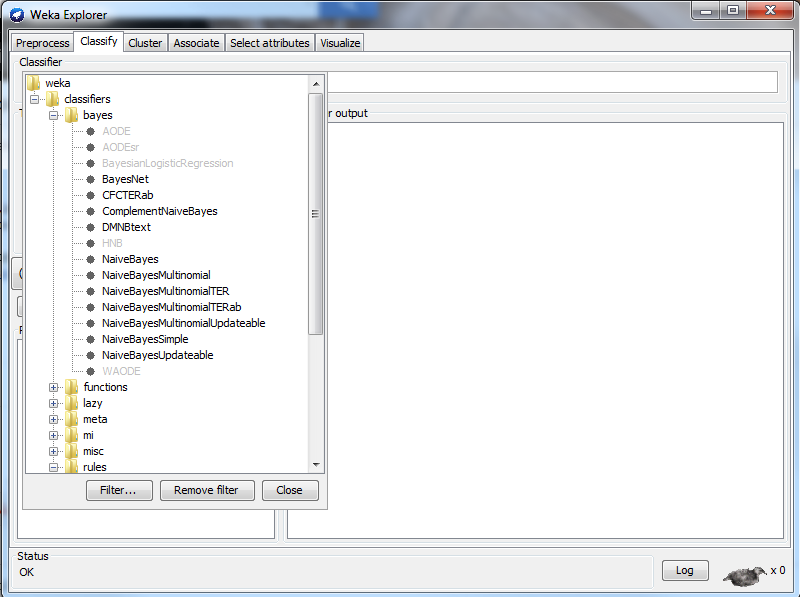
\includegraphics[width=0.80\textwidth]{wekaAlgos}~\\[1cm]  
\end{center}

La pondération de \textit{NaiveBayesMultinomialTER} se choisit à l'aide d'un menu déroulant:

\begin{center}
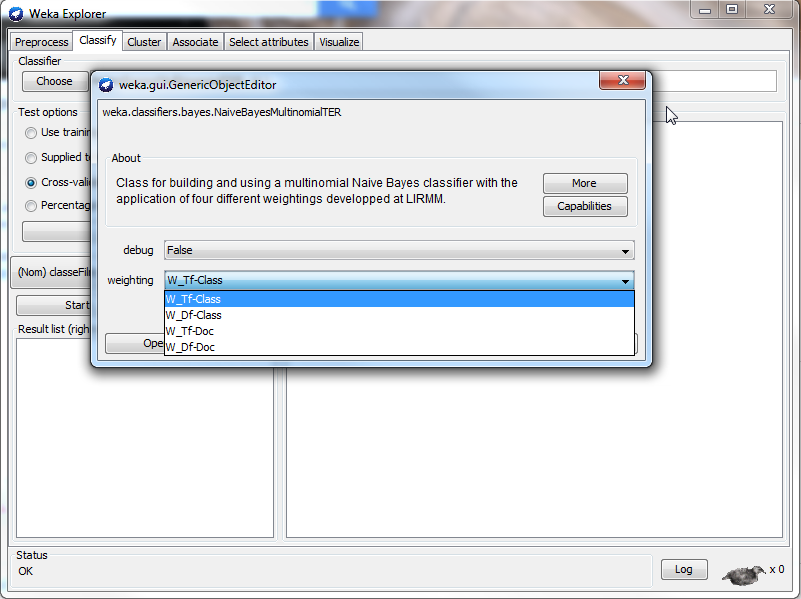
\includegraphics[width=0.75\textwidth]{wekaPond}~\\[1cm]  
\end{center}

Les valeurs de $\alpha$ et $\beta$ sont configurables dans les options de \textit{NaiveBayesMultinomialTERab} et \textit{CFCTERab}:

\begin{center}
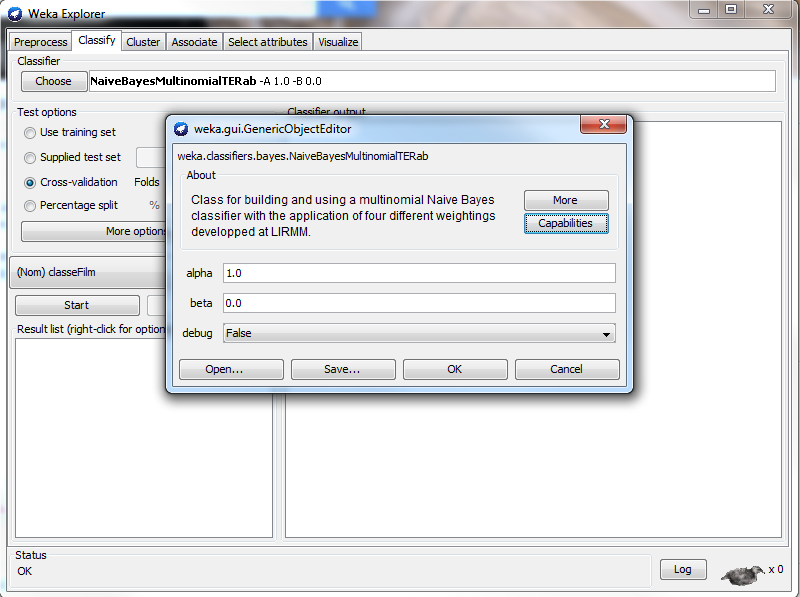
\includegraphics[width=0.75\textwidth]{wekaAB}~\\[1cm]  
\end{center}

\subsection{Tests}
Afin de tester l'exactitude des résultats de nos nouveaux algorithmes de classifications, nous avons créé un petit fichier de données aléatoires, puis nous avons calculé à la main les pondérations et comparé avec nos résultats. 

\bigskip

Pour tester la performance de nos algorithmes, nous avons utilisé des fichiers de données créés lors d'un précédent projet. Ceux-ci contiennent un grand nombre de données textuelles (résumés de films) divisées en plusieurs classes:
\begin{itemize}
\item \texttt{\textbf{test3classes.arff}} : \textbf{150} instances et \textbf{41} attributs (une selection d'attributs a été faite dessus), avec \textbf{3} classes : Policier, Fantastique, Comédie.
\item \texttt{\textbf{test5classes.arff}} : \textbf{248} instances et \textbf{5082} attributs au complet (sans selection d'attributs), avec \textbf{5} classes : Thriller, Western, Guerre, Policier, Sciences.
\end{itemize}
Le but étant de classifier les films selon leur catégorie cinématographique .
Nos deux fichiers .arff ont subi de multiples tests avec nos trois algorithmes, avec différentes valeurs pour nos variables $\alpha$ \ et $\beta$, que ce soit pour le \textit{NaiveBayesMultinomialTERab} ou le \textit{CFCTERab}.\\
Les résultats des tests sont donnés dans la section ci-dessous.

\subsection{Résultats}\label{Res}
Les deux tableaux suivants montrent les résultats relevés suite aux expérimentations effectuées avec nos trois algorithmes sur nos deux fichiers de tests.

\begin{table*}[h]
\centering
    \begin{tabular}{|l|c|c|c|c||c|}
    \hline
    NBMultinomialTER/fichierTest  & $Nb^{Tf-Class}$ & $Nb^{Df-Class}$& $Nb^{Tf-Doc}$ & $Nb^{Df-Doc}$ & NBMultinomial \\ \hline
    test3classes.arff &   66\% & \textbf{67\%}   & 64\%  & 66\% & 66\%  \\ \hline
    test5classes.arff & 52\%  & \textbf{68\%} & 51\% & 50\% & 63\%  \\ \hline
    \end{tabular}
    \caption {Expérimentations avec les quatre pondérations et comparaison avec NBMultinomial}
 \label{NBTER}
\end{table*}
\subparagraph*{•}
Le tableau \ref{NBTER} présente les résultats de classifications correctes atteintes avec distinctement les quatre pondérations $Nb^{Tf-Class}$, $Nb^{Df-Class}$, $Nb^{Tf-Doc}$ et $Nb^{Df-Doc}$ de notre algorithme  \texttt{NaiveBayesMultinomialTER}. Nous constatons que l'utilisation de la pondération $W^{Df-Class}$, pour nos deux jeux de données, donne des résultats supérieurs à ceux d'une classification avec  \texttt{NaiveBayesMultinomial}.
\begin{table*}[h]
\centering
    \begin{tabular}{|l|c|c|c|c||c|}
\hline
 Algo/FichierTest & $\alpha$ & $\beta$ & NBMTER$\alpha$$\beta$ & CFCTER$\alpha$$\beta$ & NBMultinomial \\
    \hline
    test3classes.arff &  0.0 &  1.0& \textbf{67\%} & 68\% & 66\% \\
    \cline{2-5}
         ~ &   0.6  &  0.6 & 66\% & \textbf{74\%} & ~\\
         \cline{2-5}
         ~ &   0.7  &  0.3 & 66\% & 73\% & ~\\
    \hline
     test5classes.arff &  0.0 &  1.0& \textbf{67\%} &68\% & 63\% \\
    \cline{2-5}
         ~ &   0.6  &  0.6 & 65\% & \textbf{70\%} & ~\\
         \cline{2-5}
         ~ &   0.7  &  0.3 & 58\% & 60\% & ~\\
    \hline
    \end{tabular}
    \caption {Expérimentations avec différentes valeurs de $\alpha$  \ et $\beta$ \  pour NBTER$\alpha$$\beta$ \ et CFCTER$\alpha$$\beta$ }
 \label{NBab}
\end{table*}
\subparagraph*{•}
Le tableau \ref{NBab} présente les résultats de classifications correctes atteintes avec nos deux algorithmes \texttt{NaiveBayesMultinomialTERab} et \texttt{CFCTERab}, en variant les valeurs de $\alpha$  \ et $\beta$ . Nous constatons que dans tous les cas où $\alpha$ $ \leq$ $\beta$ , on est toujours supérieurs à  \texttt{NaiveBayesMultinomial}.   Par contre, seul notre corpus réduit \texttt{test3classes.arff} donne des résultats $\geq$ à ceux de \texttt{NaiveBayesMultinomial} quand $\alpha$ \ > $\beta$ .\\
Nous constatons aussi que \texttt{CFCTER$\alpha$$\beta$} présente une meilleure classification que \texttt{NaiveBayesMultinomialTER$\alpha$$\beta$}.
%-----------------------------------------------------------




\section{Discussion et Conclusion }
Dans ce TER, nous avons produit et intégré des bibliothèques Java, implémentant des nouvelles méthodes pertinentes et validées via des prototypes au sein du laboratoire LIRMM. Ces nouvelles méthodes de classifications sont maintenant intégrées dans l'environnement Weka.
Elles peuvent être utilisées aussi bien via l'interface graphique qu'en ligne de commande. Ces nouvelles mesures sont particulièrement adaptées aux faibles volumes de données, et, comme vu au chapitre \ref{Res}, ces mesures ont été testées dans un cadre supervisé notamment via Naive Bayes (Multinomial) et une approche basée sur les centroides (CFC). \\
Les expérimentations menées aussi sur nos deux corpus de 3 et 5 classes ont permis de montrer que celles-ci ont généralement un meilleur comportement que l'approche existante de Naive Bayes Multinomial.\\
Les différents objectifs de ce TER, qui sont :\\
• Prise en main de Weka \\
• Développement des différentes bibliothèques en java \\
• L'intégration dans l’écosystème Weka \\
ont été atteints. Les difficultés principales rencontrées ont été de bien comprendre à la fois l'architecture interne et le fonctionnement de WEKA. Nous avons aussi du nous pencher sur l'intuition portée par les nouvelles mesures. Ces deux défis ont axé et constitué la ligne directrice de notre travail, dans lequel nous avons mené une étude bibliographique sur l'article scientifique présentant la nouvelle méthodologie \cite{RNTIB}, ainsi qu'un parcours approfondi de la documentation de WEKA(cf. Wiki de Weka \ref{weka}).
%-----------------------------------------------------------

\newpage
\section{Sources}
\begin{itemize}
\item Wiki de Weka \label{weka}: \href{http://weka.wikispaces.com/Writing+your+own+Classifier}{http://weka.wikispaces.com/Writing+your+own+Classifier}
 \\
\item Naive Bayes  : \href{$http://scikit-learn.org/stable/modules/naive_bayes.html$}{http://scikit-learn.org/stable/modules/naive\_bayes.html}


\end{itemize}

%-----------------------------------------------------------
\bibliographystyle{plain}
\bibliography{biblio}
\end{document}

%%% Local Variables:
%%% mode: latex
%%% TeX-master: t
%%% coding: utf-8
%%% End:
